\chapter{Funciones y modelos}
\begin{tcolorbox}[colframe=white]
    %--------------------definición 1.1.
    \begin{def.}
	Una \textbf{función} $f$ es una regla que asigna a cada elemento $x$ de un conjunto $D$ exactamente un elemento, llamado $f(x)$, de un conjunto $E$.
	$$\lbrace (x,f(x)) / x \in D \rbrace$$
	la función $f$ consta de todos los puntos $(x,y)$ en el plano coordenado tales que $y=f(x)$ y $x$ está en el dominio de $f$
    \end{def.}
\end{tcolorbox}

    %-------------------definición 1.2.
\begin{tcolorbox}[colframe=white]
    \begin{def.}
	Una función se llama \textbf{creciente} sobre un intervalo $l$ si
	\begin{center}
	    $f(x_1)<f(x_2)$ siempre que $x_1<x_2$ en $l$
	\end{center}
	Se llama \textbf{decreciente} sobre $l$ si
	\begin{center}
	    $f(x_1)>f(x_2)$ siempre que $x_1< x_2$ en $l$
	\end{center}
    \end{def.}
\end{tcolorbox}

\section{Ejercicios}
    
    \begin{enumerate}[\Large \bfseries 1.]
	
    %--------------------1.
    \item Si $f(x)=x + \sqrt{2-x}$ y $g(u)=u+\sqrt{2-u}$. ¿Es verdad que $f=g$?\\\\
    Respuesta.-\; Es verdad ya que no afecta en nada el símbolo que se podría colocar a la variable dependiente.\\\\
	
	%--------------------2.
	\item Si $f(x)=\dfrac{x^2-x}{x-1}$ y $g(x)=x$ ¿Es verdad que $f=g$?\\\\
	Respuesta.-\; No es verdad ya que el dominio de la función $g$ son todos los reales contrariamente a la función $f$ que no se cumple para $x=1$\\\\

	%--------------------3.
	\item La gráfica de una función $f$ está dada.
	    \begin{enumerate}[\bfseries (a)]
		    %----------(a)
		    \item Indique el valor de $f(1)$\\\\
		    Respuesta.-\; El valor es $3$\\\\ 

		    %----------(b)
		    \item Calcule el valor de $f(-1)$\\\\
		    Respuesta.-\; El valor es $-0.3$ aproximadamente.\\\\

		    %----------(c)
		    \item ¿Para qué valores de $x$ es $f(x)=1$?\\\\
		    Respuesta.-\;Por definición solo se cumple para $0$\\\\

		    %----------(d)
		    \item Calcule el valor de $x$ tal que $f(x)=0$\\\\
		    Respuesta.-\; El valor es aproximadamente $-0.7$\\\\ 

		    %----------(e)
		    \item Indique el dominio y el rango de $f$\\\\
		    Respuesta.-\; $f_D=\lbrace x \in f_D / -2 \leq x \leq 4 \rbrace$, y $f_R=\lbrace y \in f_R / -1 \leq y \leq 3 \rbrace$\\\\

		    %----------(f)
		    \item ¿En qué intervalo $f$ es creciente?\\\\
		    Respuesta.-\; Es creciente en el intervalo $[-2,1]$\\\\ 

	    \end{enumerate}

    %--------------------4.
    \item Las gráficas de $f$ y $g$ están dadas.

	\begin{enumerate}[\bfseries (a)]

	    %----------(a)
	    \item Indique los valores de $f(-4)$ y $g(3)$\\\\
		Respuesta.-\; $f(-4)=-2$ y $g(3)=4$\\\\

	    %----------(b)
	    \item ¿Para qué valores de $x$ es $f(x)=g(x)$?\\\\
		Respuesta.-\; Para $2,$ y $-2$\\\\ 

	    %----------(c)
	    \item Estime la solución de la ecuación $f(x)=-1$\\\\
		Respuesta.-\; $x=-3$\\\\

	    %----------(d)
	    \item ¿Sobre qué intervalo $f$ es decreciente?\\\\ 
		Respuesta.-\; Sobre $[0,4]$\\\\

	    %----------(e)
	    \item Establezca el dominio y el rango de $f$\\\\
		Respuesta.-\; El dominio de $f$ es $[-4,4]$ y el rango de $[-2,3]$\\\\

	    %----------(f)
	    \item Establezca el dominio y el rango de $g$\\\\
		Respuesta.-\; El dominio es de $[-4,3]$ y el rango de $[0.5,4]$\\\\

	\end{enumerate}

    %--------------------5.
    \item La gráfica de la figura $1$ fue registrada por un instrumento operado por el departamento de minas y geología de California en el hospital Universitario de California del Sur de Los Ángeles. Utilice esta gráfica para estimar el rango de la función aceleración vertical de suelo, en la Universidad de California del Sur, durante el terremoto de Northridge.\\\\
	Respuesta.-\; El rango de la función de aceleración  vertical del suelo es dado por el intervalo $[-1,3]$\\\\ 

    %--------------------6.
    \item En esta sección se discuten ejemplos de funciones cotidianas: la población es una función del tiempo, el costo, de envío postal es una función del peso, la temperatura del agua es una función del tiempo. De otros tres ejemplos de funciones de la vida cotidiana que se describen verbalmente. ¿Qué puede decir sobre el dominio y el rango de cada una de sus funciones? Si es posible, trace una gráfica de cada función.\\\\
	Respuesta.-\; 

    %--------------------7.
    \item No cumple con la definición de función.\\\\

    %--------------------8.
    \item Cumple con la definición de función por lo tanto $f_D=\lbrace x / -2 \leq x \leq 2 \rbrace$ y $f_R=\lbrace y \in f(x) / -1 \leq y \leq 2 \rbrace$\\\\

    %--------------------9.
    \item Cumple con la definición de función por lo tanto $f_D=\lbrace x / -3 \leq x < -2 \; \cup \; -2 \leq x \leq 2 \rbrace$ y $f_R=\lbrace y \in f(x) / -3 \leq x < -2 \; \cup \; -2 \leq y \leq 2.6 \rbrace$\\\\

    %--------------------10.
    \item No cumple con la definición de función por lo tanto no se tiene un dominio y rango.\\\\

    %--------------------11.
    \item En la figura se muestra una gráfica de la temperatura media global $T$ durante el siglo $XX$. Estime lo siguiente.
	\begin{enumerate}[\bfseries (a)]

	    %----------(a)
	    \item La temperatura media mundial en $1950$\\\\
		Respuesta.-\; 14.5 grados centígrados.\\\\

	    %----------(b)
	    \item El año en que la temperatura promedio fue de $14.2$ C.\\\\
		Respuesta.-\; Aproximadamente en $1905$\\\\

	    %----------(c)
	    \item ¿En qué año la temperatura fue más baja? ¿Más alta?\\\\
		Respuesta.-\; Fue más baja en $1920$ y más alta en $2010$\\\\

	    %----------(d)
	    \item El rango de $T$\\\\
		Respuesta.-\; El rango se encuentra en el intervalo de $[12.8,14.8]$\\\\ 

	\end{enumerate}

    %--------------------12.
    \item Los arboles crecen más rápido y forman anillos más amplios en los años cálidos y crecen más lentamente y forman anillos más angostos en los años más fríos. La figura muestra anillos anchos del pino Siberiano de $1500$ a $2000$.

	\begin{enumerate}[\bfseries (a)]

	    %----------(a)
	    \item ¿Cuál es el rango de la función de ancho de anillo?\\\\
		Respuesta.-\; El rango es de $0.1$ a $1.41$ aproximadamente.\\\\

	    %----------(b)
	    \item ¿Qué dice la gráfica acerca de la temperatura de la tierra? ¿La gráfica refleja las erupciones volcánicas de la mitad del siglo $XIX$?\\\\
		Respuesta.-\; La temperatura cada vez es más cálida mientras pasa los años. \\
		Se ve un pequeño realce entre $1800-1890$ donde podría haber existido algunas erupciones volcánicas.\\\\

	\end{enumerate}

    %--------------------13.
    \item Se ponen unos cubitos de hielo en un vaso, se llena el vaso con agua fría y luego se coloca sobre una mesa. Describa cómo cambia la temperatura del agua conforme transcurre el tiempo. Luego trace una gráfica de la temperatura del agua como una función del tiempo transcurrido.\\\\
    Respuesta.-\; La temperatura va disminuyendo constantemente en función a la temperatura ambiente y del tiempo.

            \begin{center}
                \begin{tikzpicture}[scale=0.9, draw opacity = .6]
                    % abscisa y ordenada
                    \tkzInit[xmax= 3,xmin=-2,ymax=3,ymin=-2]
                    \tiny\tkzLabelXY[opacity=0.6,step=1, orig=false]
                    % label x, f(x)
                    \tkzDrawX[opacity= .6,label=x,right=0.3]
                    \tkzDrawY[opacity= .6,label=f(x),below = -0.6]
                    %dominio y función
                    \draw [domain=-2:3,thick] plot(\x,{\x}); 
                \end{tikzpicture}
            \end{center}  

    %--------------------14.
    \item Tres corredores compiten en una carrera de $100$ metros. La gráfica muestra la distancia recorrida como una función del tiempo de cada corredor. Describa en palabras lo que la gráfica indica acerca de esta carrera. ¿Quién ganó la carrera? ¿Cada corredor terminó la carrera?\\\\
    Respuesta.-\; Gano la carrera el competidor $A$. Efectivamente cada competidor acabo la carrera.\\\\ 

    %--------------------15.
    \item La gráfica muestra el consumo de energía para un día de septiembre en San Francisco. ($P$ se mide en megawatts: $t$ se registra en horas a partir de la medianoche).

	\begin{enumerate}[\bfseries (a)]

	    %----------(a)
	    \item ¿Cual fue el consumo de potencia a las $6:00$? ¿A las $18:00$?\\\\
	    Respuesta.-\; Para las $6:00$ el consumo de potencia es $500$ megawatts. y para las $18:00$ es $720$ megawatts.\\\\

	    %----------(b)
	    \item ¿Cuándo fue el consumo de energía más bajo? ¿Cuándo fue el más alto? ¿Estos tiempos parecen razonables?\\\\
	    Respuesta.-\; El más bajo fue a hrs. $4:00$ y el mas alto fue en a hrs. $12:00$. Los tiempos son razonables por la actividad que se puede realizar a esas horas.\\\\

	\end{enumerate}

    %--------------------16.
    \item Trace una gráfica aproximada del número de horas de luz en función de la época del año.\\\\

    %--------------------17.
    \item Trace una gráfica de la temperatura exterior en función del tiempo, durante un día típico de primavera.\\\\

    %--------------------18.
    \item Trace una gráfica aproximada del valor de mercado de un nuevo automóvil en función del tiempo, durante un periodo de $20$ años. Suponga que el automóvil se mantiene en buen estado.\\\\

    %--------------------19.
    \item Trace la gráfica de la cantidad de una determinada marca de café vendido por una tienda en función del precio del café.\\\\

    %--------------------20.
    \item Coloque una tarta congelada en un horno y caliéntela durante una hora. Luego sáquela y déjela enfriar antes de comerla. Describa cómo cambia la temperatura de la tarda conforme pasa el tiempo. Luego trace una gráfica de la temperatura de la tarta en función del tiempo.\\\\

    %--------------------21.
    \item El propietario de una casa poda el césped cada miércoles por la tarde. Trace una gráfica de la altura del césped como una función del tiempo, en el transcurso de un periodo de cuatro semanas.

            \begin{center}
                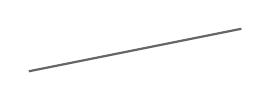
\begin{tikzpicture}[scale=0.9, draw opacity = .6]
                    % abscisa y ordenada
                    \tkzInit[xmax= 3,xmin=-1,ymax=1,ymin=-1]
                    \tiny\tkzLabelXY[opacity=0.6,step=1, orig=false]
                    % label x, f(x)
                    \tkzDrawX[opacity= .8,label=tiempo,right=0.3]
                    \tkzDrawY[opacity= .6,label=Tamaño cesped,below = -0.6]
                    %dominio y función
                    \draw [domain=0:3,thick] plot(\x,{.2*\x}); 
                \end{tikzpicture}
            \end{center}  

    %--------------------22.
	\item  Un avión despega desde un aeropuerto y aterriza una hora más tarde en otro aeropuerto a $400$ km de distancia. Si $t$ representa el tiempo en minutos desde que el avión ha dejado la terminal. $x(t)$ es la distancia horizontal recorrida y $y(t)$ la altitud del avión, trace
	    \begin{enumerate}[\bfseries (a)]

		    %----------(a)
		\item Una posible gráfica de $x(t)$\\

		    %----------(b)
		\item Una posible gráfica de $y(t)$\\\\

		    %----------(c)
		\item Una posible gráfica de la rapidez respecto al suelo.\\\\

		    %----------(d)
		\item Una posible gráfica de la velocidad vertical.\\\\

	    \end{enumerate}

    %--------------------23.
	\item La siguientes lecturas de temperatura $T$ (en $C^{\circ}$) se registraron cada tres horas desde la medianoche a las $15:00$ en Montreal, el $13$ de junio de $2004$. El tiempo $t$ se midió en horas a partir de la medianoche.

	    \begin{enumerate}[\bfseries (a)]

		%----------(a)
		\item Utilice las lecturas para trazar una gráfica de $T$ como una función de $t$.\\\\

		%-----------(b)
		\item Utilice la gráfica para estimar la temperatura a las $11:00$\\\\

	    \end{enumerate}

    %--------------------24.
    \item Los investigadores midieron la concentración de alcohol en la sangre de ocho sujetos masculinos adultos después de consumir en forma rápida $30$ mL de etanol. La tabla muestra los datos que se obtubieron promediando la $BAC$ de los ocho hombres.

	\begin{enumerate}[\bfseries (a)]

	    %----------(a)
	    \item Utilice las lecturas para trazar la gráfica de la BAC en función de t.\\\\

	    %----------(b)
	    \item Utilice la gráfica para describir cómo el efecto del alcohol varía con el tiempo.\\\\

	\end{enumerate}

    %--------------------25.
    \item Si $f(x)2x^2 - x + 2$, determine $f(2),\; f(-2),\; f(a),\; f(-a),\; f(a+1),\; 2f(a),\; f(2a),\; f(a^2),\; [f(a)^2], \; y \; f(a+h)$\\\\
    Respuesta.-\; 
    \begin{center}
	\begin{tabular}{rcl}
	    $f(2)$ & $=$ & $2\cdot 2^2 - 2 + 2 = 8$\\
	     $f(-2)$ & $=$ & $2\cdot(-2)^2 + 2 +2 =12$\\
	     $f(a)$ & $=$ & $2a^2 - a + 2$\\
	     $f(-a)$ & $=$ & $2(-a)^2 - (-a) + 2$\\
	     $f(a+1)$ & $=$ & $2(a+1)^2 - (a+1) + 2$\\
	     $2f(a)$ & $=$ & $2(2a^2 - a + 2)$\\
	     $f(2a)$ & $=$ & $2(2a)^2 - 2a 2$\\
	     $f(a^2)$&$=$&$2(a^2)^2 - a^2 + 2$\\
	     $f(a)^2$&$=$&$(2a^2 + a - 2)^2$\\
	     $f(a+h)$&$=$&$2(a+h)^2 - (a+h) + 2$\\\\
	\end{tabular}
    \end{center}

    %--------------------26.
\item Un globo esférico con radio de $r$ centímetros tiene volumen $V(r)=\dfrac{4}{3}\pi r^3$. Encuentre una función que represente la cantidad de aire necesaria para inflar el globo de un radio de $r$ centímetros a un radio $r+1$ centímetros.\\\\
    Respuesta.-\; $V(r+1)=\dfrac{4}{3}\pi (r+1)^3$\\\\

     $(27-30)$ Evalúe el cociente de diferencia de cada una de las siguientes funciones. Simplifique su respuesta.\\\\

    %--------------------27.
    \item $f(x)=4+3x-x^2, \;\;\;\; \dfrac{f(3+h)-f(3)}{h}$\\\\
	Respuesta.-\; Se tiene $$\dfrac{4 + 3(3+h)-(3+h)^2-4+9-9}{h}=\dfrac{9+3h-9-6h-h^2}{h}=\dfrac{-h^2 -3h}{h}=-(h+3)$$\\\\

    %--------------------28.
    \item $f(x)=x^3, \;\;\;\; \dfrac{f(a+h)-f(a)}{h}$\\\\
	Respuesta.-\; $\dfrac{(a+h)^3 - a^3}{h}=\dfrac{a^3 + 3a^2h + 3ah^3 + h^3 - a^3}{h}=\dfrac{3a^2h + 3ah^2 + h^3}{h}=h^2 + 3a^2 + 3ah$\\\\ 

    %--------------------29.
    \item $f(x)=\dfrac{1}{x}, \qquad \dfrac{f(x) - f(a)}{x-a}$\\\\
	Respuesta.-\; $$\dfrac{\dfrac{1}{x} - \dfrac{1}{a}}{x-a} = \dfrac{\dfrac{a-x}{xa}}{x-a}=\dfrac{-(x-a)}{xa(x-a)}=-\dfrac{1}{xa}$$\\\ 

    %--------------------30.
    \item $f(x)=\dfrac{x+3}{x+1}, \qquad \dfrac{f(x)-f(1)}{x-1}$\\\\
	Respuesta.-\; $$\dfrac{\dfrac{x+3}{x+1}-2}{x-1} = \dfrac{\dfrac{x+3 - 2(x+1)}{x+1}}{x-1}=\dfrac{\dfrac{-x-1}{x+1}}{x-1}=\dfrac{-(x+1)}{(x+1)(x-1)}=\dfrac{-1}{x-1}$$\\\\

    $31-37$ Encuentre el dominio de cada una de las funciones siguientes.\\

    %--------------------31.
    \item $f(x)=\dfrac{x+4}{x^2 - 9}$\\\\
	Respuesta.-\; Debemos tomar en cuenta que no podemos dividir por $0$. Por lo tanto igualamos el denominador a $0$. $$x^2-9=0 \Rightarrow (x-3)(x+3)=0$$ entonces el dominio esta dado por todo $x - \lbrace -3,3\rbrace$\\\\  

    %--------------------32
    \item $f(x)=\dfrac{2x^3-5}{x^2+x-6}$\\\\
	Respuesta.-\; Ponemos a prueba $$x^2+x-6,$$ entonces $(x+2)(x-3)=0$ por lo tanto El dominio esta dado para todo $x - \lbrace -2,3\rbrace$\\\\

    %--------------------33
    \item $f(t)=\sqrt[3]{2t-1}$ \\\\
	Respuesta.-\: El dominio es dado para todo $x$, ya que la raíz cubica puede ser evaluada para número no positivos.\\\\

    %--------------------34
    \item $g(t)=\sqrt{3-y}-\sqrt{2+t}$ \\\\
	Respuesta.-\: Evaluamos raíces cuadradas para números no negativos por lo tanto, $3-t\geq 0; \quad 2+t\geq 0$ entonces el dominio de la función esta dado por  $-2\leq t\leq 3$.\\\\

    %--------------------35
    \item $h(x)=\dfrac{1}{\sqrt[4]{x^2-5x}}$ \\\\
	Respuesta.-\: Sea $x^2-5x \geq 0$, de donde $x(x-5)\geq 0$, así, $x\geq 0 \land x-5\geq 0 \, \lor \, x\leq 0 \land x-5\leq 0$, por lo tanto el dominio esta dado por $x\leq 0 \lor x\geq 5$.\\\\ 

    %--------------------36
    \item $f(u)=\dfrac{u+1}{1+\dfrac{1}{u+1}}$ \\\\
	Respuesta.-\: Primeramente evaluamos $u+1=0$, entonces $u=-1$, luego evaluamos $1+\dfrac{1}{u+1}=0$, de donde $u=-2$, por lo tanto $\lbrace x/x\neq =-1,-2\rbrace$\\\\

    %--------------------37
    \item $F(p)=\sqrt{2 - \sqrt{p}}$ \\\\
	Respuesta.-\: Evaluamos primero $\sqrt{p}$ de donde  $p\geq 0$ luego evaluamos $\sqrt{2 - \sqrt{p}}\geq 0$, así $p\leq 4$ por lo tanto el dominio esta dado por $0\leq x \leq 4$\\\\

    %--------------------38
    \item Encuentre el dominio y el rango, y dibuje la gráfica de la función $h(x)=\sqrt{4-x^2}$\\\\
	Respuesta.-\; Evaluamos el dominio de la función, $$4-x^2 \geq 0 \Rightarrow -(x^2-4) \geq 0 \Rightarrow x^2 -4  \leq 0 \Rightarrow (x-2)(x+2) \leq 0$$ por lo tanto el dominio esta dado por  $\lbrace x / -2 \leq x \leq 2 \rbrace$.\\ 
	Luego es fácil evaluar el rango, $\lbrace f(x) / 0\leq f(x) \leq 2 \rbrace$

	\begin{center}
	    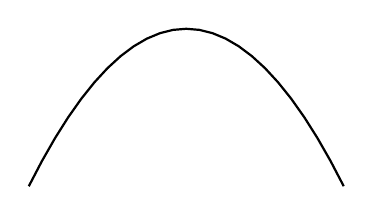
\begin{tikzpicture}
		% abscisa y ordenada
		\tkzInit[xmax= 3,xmin=-3,ymax=3,ymin=-1]
		\tiny\tkzLabelXY[opacity=0.6,step=1, orig=false]
		% label x, f(x)
		\tkzDrawX[opacity= .6,label=x,right=0.3]
		\tkzDrawY[opacity= .6,label=f(x),below = -0.6]
		%dominio y función
		\draw [domain=-2:2,thick] plot(\x,{(4-\x*\x)*(1/2}); 
	    \end{tikzpicture}
	\end{center}

    $39-40$ Encuentre el dominio y grafique cada una de las funciones siguientes:\\\\

    %--------------------39.
    \item $f(x)=1.6x-2.4$\\\\
	Respuesta.-\; El dominio viene dado por todos los reales.

	\begin{center}
	    \begin{tikzpicture}
		% abscisa y ordenada
		\tkzInit[xmax= 2,xmin=-3,ymax=1,ymin=-5]
		\tiny\tkzLabelXY[opacity=0.6,step=1, orig=false]
		% label x, f(x)
		\tkzDrawX[opacity= .6,label=x,right=0.3]
		\tkzDrawY[opacity= .6,label=f(x),below = -0.6]
		%dominio y función
		\draw [domain=-2:3,thick] plot(\x,{1.6*\x -2.4}); 
	    \end{tikzpicture}
	\end{center}
	\vspace{.5cm}

    %--------------------40.
    \item $g(t)=\dfrac{t^2-1}{t+1}$\\\\
	Respuesta.-\; El dominio esta dado por $\lbrace x / x \neq -1\rbrace$

	\begin{center}
	    \begin{tikzpicture}
		% abscisa y ordenada
		\tkzInit[xmax= 3,xmin=-1,ymax=2,ymin=-2]
		\tiny\tkzLabelXY[opacity=0.6,step=1, orig=false]
		% label x, f(x)
		\tkzDrawX[opacity= .6,label=x,right=0.3]
		\tkzDrawY[opacity= .6,label=f(x),below = -0.6]
		%dominio y función
		\draw [domain=-0.99:3,thick] plot(\x,{(\x*\x -1)/(\x + 1)}); 
	    \end{tikzpicture}
	\end{center}
	\vspace{.5cm}

    $41-44$ Evalúe $f(-3), f(0)$ y $f(2)$ para la función definida por partes. Luego trace la gráfica de la función.\\\\

    %--------------------41.
    \item $f(x)= \left\{ \begin{array}{lcr}
		     x+2 &   si  & x<0 \\
		     \\ 1-x &  si & x \geq 0 \\
		 \end{array} \right.$ \\\\

	Respuesta.-\; \\
	
	\begin{itemize}
	    \item $f(-3) = x+2 = -3+2 = -1$.
	    \item $f(0) = 1-x = 1-0 = 1$.
	    \item $f(2) = 1-x = 1 - 2 = -1$.
	\end{itemize}

	\begin{center}
	    \begin{tikzpicture}
		% abscisa y ordenada
		\tkzInit[xmax= 3,xmin=-3,ymax=2,ymin=-2]
		\tiny\tkzLabelXY[opacity=0.6,step=1, orig=false]
		% label x, f(x)
		\tkzDrawX[opacity= .6,label=x,right=0.3]
		\tkzDrawY[opacity= .6,label=f(x),below = -0.6]
		%dominio y función
		\draw [domain=-3:0,thick] plot(\x,{\x + 2}); 
		\draw [domain=0:3,thick] plot(\x,{1 - \x}); 
	    \end{tikzpicture}
	\end{center}
	\vspace{.5cm}

    %--------------------42.
    \item $f(x)= \left\{ \begin{array}{lcr}
		    3 - \frac{1}{2}x &   si  & x<2 \\
		     \\ 2x - 5  &  si & x \geq 2 \\
		 \end{array} \right.$ \\\\
	
	Respuesta.-\; \\

	\begin{itemize}
	    \item $f(-3)=3 - \frac{1}{2}x = 3 - \frac{1}{2}(-3) = \frac{9}{2}$.
	    \item $f(0)= 3 - \frac{1}{2}x = 3 - \frac{1}{2}(0) = 3$.
	    \item $f(2)= 2x - 5 = 2\cdot 2 - 5 = -1$.
	\end{itemize}

	\begin{center}
	    \begin{tikzpicture}
		% abscisa y ordenada
		\tkzInit[xmax= 4,xmin=-3,ymax=5,ymin=-2]
		\tiny\tkzLabelXY[opacity=0.6,step=1, orig=false]
		% label x, f(x)
		\tkzDrawX[opacity= .6,label=x,right=0.3]
		\tkzDrawY[opacity= .6,label=f(x),below = -0.6]
		%dominio y función
		\draw [domain=-3:1.99,thick] plot(\x,{3 - 0.5*\x}); 
		\draw [domain=2:4,thick] plot(\x,{2*\x - 5}); 
	    \end{tikzpicture}
	\end{center}
	\vspace{.5cm}

    %--------------------43.
    \item $f(x)= \left\{ \begin{array}{lcr}
		    x + 1 &   si  & x \leq -1 \\
		     \\ x^2  &  si & x > -1 \\
		 \end{array} \right.$ \\\\
	
	Respuesta.-\; \\

	\begin{itemize}
	    \item $f(-3)= x+1 = -3+1 = -2$.
	    \item $f(0) = x^2 = 0^2 = 0$.
	    \item $f(2) = x^2 = 2^2 = 4$.
	\end{itemize}

	\begin{center}
	    \begin{tikzpicture}
		% abscisa y ordenada
		\tkzInit[xmax= 2,xmin=-3,ymax=2,ymin=-2]
		\tiny\tkzLabelXY[opacity=0.6,step=1, orig=false]
		% label x, f(x)
		\tkzDrawX[opacity= .6,label=x,right=0.3]
		\tkzDrawY[opacity= .6,label=f(x),below = -0.6]
		%dominio y función
		\draw [domain=-3:-1,thick] plot(\x,{\x + 1}); 
		\draw [domain=-1:1.5,thick] plot(\x,{\x * \x}); 
	    \end{tikzpicture}
	\end{center}
	\vspace{.5cm}

    %--------------------44.
    \item $f(x)= \left\{ \begin{array}{lcr}
		    -1 &   si  & x\leq 1 \\
		     \\ 7 - 2x  &  si & x > 1 \\
		 \end{array} \right.$ \\\\
	
	Respuesta.-\; \\

	\begin{itemize}
	    \item $f(-3)= -1$.
	    \item $f(0) = -1$.
	    \item $f(2) = 7-2x = 7-2\cdot 2 = 3$.
	\end{itemize}

	\begin{center}
	    \begin{tikzpicture}
		% abscisa y ordenada
		\tkzInit[xmax= 3,xmin=-3,ymax=1,ymin=-2]
		\tiny\tkzLabelXY[opacity=0.6,step=1, orig=false]
		% label x, f(x)
		\tkzDrawX[opacity= .6,label=x,right=0.3]
		\tkzDrawY[opacity= .6,label=f(x),below = -0.6]
		%dominio y función
		\draw [domain=-3:1,thick] plot(\x,{-1}); 
		\draw [domain=1:3,thick] plot(\x,{1 - \x}); 
	    \end{tikzpicture}
	\end{center}
	\vspace{.5cm}

    $45-50$ Trace la gráfica de la función.\\\\

    %--------------------45.
    \item $f(x)=x+|x|$\\\\
	Respuesta.-\; 

	\begin{center}
	    \begin{tikzpicture}
		% abscisa y ordenada
		\tkzInit[xmax= 3,xmin=-3,ymax=4,ymin=-1]
		\tiny\tkzLabelXY[opacity=0.6,step=1, orig=false]
		% label x, f(x)
		\tkzDrawX[opacity= .6,label=x,right=0.3]
		\tkzDrawY[opacity= .6,label=f(x),below = -0.6]
		%dominio y función
		\draw [domain=-2:2,thick] plot(\x,{\x + abs(\x)}); 
	    \end{tikzpicture}
	\end{center}
	\vspace{.5cm}

    %--------------------46.
    \item $f(x)=|x+2|$\\\\
	Respuesta.-\; 

	\begin{center}
	    \begin{tikzpicture}
		% abscisa y ordenada
		\tkzInit[xmax= 3,xmin=-3,ymax=4,ymin=0]
		\tiny\tkzLabelXY[opacity=0.6,step=1, orig=false]
		% label x, f(x)
		\tkzDrawX[opacity= .6,label=x,right=0.3]
		\tkzDrawY[opacity= .6,label=f(x),below = -0.6]
		%dominio y función
		\draw [domain=-2:2,thick] plot(\x,{abs(\x + 2)}); 
	    \end{tikzpicture}
	\end{center}
	\vspace{.5cm}

    %--------------------47.
    \item $g(t)=|1-3t|$\\\\
	Respuesta.-\;

	\begin{center}
	    \begin{tikzpicture}
		% abscisa y ordenada
		\tkzInit[xmax= 3,xmin=-3,ymax=6,ymin=0]
		\tiny\tkzLabelXY[opacity=0.6,step=1, orig=false]
		% label x, f(x)
		\tkzDrawX[opacity= .6,label=x,right=0.3]
		\tkzDrawY[opacity= .6,label=f(x),below = -0.6]
		%dominio y función
		\draw [domain=-2:2,thick] plot(\x,{abs(1 - 3*\x)}); 
	    \end{tikzpicture}
	\end{center}
	\vspace{.5cm}

    %--------------------48.
    \item $h(t)=|t|+|t+1|$\\\\
	Respuesta.-\; \\

	\begin{center}
	    \begin{tikzpicture}
		% abscisa y ordenada
		\tkzInit[xmax= 3,xmin=-3,ymax=2,ymin=0]
		\tiny\tkzLabelXY[opacity=0.6,step=1, orig=false]
		% label x, f(x)
		\tkzDrawX[opacity= .6,label=x,right=0.3]
		\tkzDrawY[opacity= .6,label=f(x),below = -0.6]
		%dominio y función
		\draw [domain=-2.5:2.5,thick] plot(\x,{abs(\x) + abs(\x+1)}); 
	    \end{tikzpicture}
	\end{center}
	\vspace{.5cm}

    %--------------------49.
    \item $f(x) = \left\{ \begin{array}{lcr}
	    |x| & si & |x| \leq 1 \\
	    \\ 1 & si & |x| > 1 \\
	\end{array} \right.$ \\\\

	Respuesta.-\; 

	\begin{center}
	    \begin{tikzpicture}
		% abscisa y ordenada
		\tkzInit[xmax= 3,xmin=-3,ymax=2,ymin=-1]
		\tiny\tkzLabelXY[opacity=0.6,step=1, orig=false]
		% label x, f(x)
		\tkzDrawX[opacity= .6,label=x,right=0.3]
		\tkzDrawY[opacity= .6,label=f(x),below = -0.6]
		%dominio y función
		\draw [domain=-2:1,thick] plot(\x,{abs(\x)}); 
		\draw [domain=0.99:3,thick] plot(\x,{1}); 
	    \end{tikzpicture}
	\end{center}
	\vspace{.5cm}

    %--------------------50.
    \item $g(x)=||x|-1|$\\\\
	Respuesta.-\; 
	\begin{center}
	    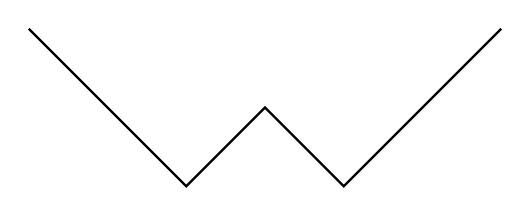
\begin{tikzpicture}
		% abscisa y ordenada
		\tkzInit[xmax= 3,xmin=-3,ymax=2,ymin=0]
		\tiny\tkzLabelXY[opacity=0.6,step=1, orig=false]
		% label x, f(x)
		\tkzDrawX[opacity= .6,label=x,right=0.3]
		\tkzDrawY[opacity= .6,label=f(x),below = -0.6]
		%dominio y función
		\draw [domain=-3:3,thick] plot(\x,{abs(abs(\x) - 1)}); 
	    \end{tikzpicture}
	\end{center}
	\vspace{.5cm}

    $51-56$ Encuentre una expresión para la función cuya gráfica es la curva dada.\\\\

    %--------------------51.
    \item El segmento de recta que une los puntos $(1,-3)$ y $(5,7)$\\\\
	Respuesta.-\; el segmento viene dado por la ecuación $f(x)ax+b$ donde $a$ es la pendiente y $b$ el punto de corte. Formando un sistemas de ecuaciones con el primero y segundo punto respectivamente se tiene $$ -3 = a + b \qquad y \qquad 7= 5a + b,$$ operando nos queda que  $a=\dfrac{10}{4}$ y $b=- \dfrac{11}{2}$, por lo tanto la función viene dado por $f(x)=\dfrac{5}{2}x - \dfrac{11}{2}$.\\\\

    %--------------------52.
    \item El segmento de recta que une los puntos $(-5,10)$ y $(7,-10)$\\\\
	Respuesta.-\; Similar al anterior ejercicio tenemos las ecuaciones $$10=-5a+b \qquad y \qquad -10=7a+b$$ de donde $a=-\dfrac{5}{3}$ y $b=\dfrac{5}{3}$ y por lo tanto $$f(x)=-\dfrac{5}{3}x + \dfrac{5}{3}$$\\\\

    %--------------------53.
    \item La mitad inferior de la parabola $x+(y-1)^2 = 0$\\\\
	Respuesta.-\; Se tiene $(y-1)^2 = -x \Longrightarrow y=\pm \sqrt{-x} + 1$, luego la mitad inferior esta dada por $y=- \sqrt{-x} +1$\\\\

    %--------------------54.
    \item La mitad inferior de la circunferencia $x^2 + (y-2)^2 = 4$\\\\
	Respuesta.-\; Se tiene $(y-2)^2 = 4 -x^2 \Longrightarrow y = \pm \sqrt{5-x^2} + 2$, por lo tanto la parte superior de la circunferencia esta dado por $y=\sqrt{5-x^2} + 2$\\\\

    %--------------------55.
    \item Respuesta.-\;  \begin{center}$ f(x) = \left\{ \begin{array}{rcl}
	    -x+3&si&0 \leq x \leq 3\\
	    \\ 2x-6&si&3<x\leq 5\\\\
    \end{array} \right.$ \end{center}

    %--------------------56.
    \item Respuesta.-\;  \begin{center}$ f(x) = \left\{ \begin{array}{rcl}
	    2/3 x + 3&si&-4\leq x \leq -2\\
	    \\ \sqrt{2-x^2}&si& -2 < x < 2\\
	    \\ 2/3x-3&si& 2\leq x \leq 4\\\\
    \end{array} \right.$ \end{center}
    \vspace{.5cm}
 
    $57-61$ Encuentre una fórmula y el dominio para cada una de las funciones siguientes.\\\\

    %--------------------57.
    \item Un rectángulo tiene $20$ m de perímetro. Exprese el área del rectágulo en función de la longitud de uno de sus lados.\\\\
	Respuesta.-\; Sea $A_{rec} = b\cdot h$ el área de un rectángulo y $2b+2h=20$ el perímetro. Entonces $h=10-b$ por lo tanto $A_{rec}=b(10-b)$\\\\  

    %--------------------58.
    \item Un rectángulo tiene $16\; m^2$  de área. Exprese el perímetro del rectángulo en función de la longitud de uno de sus lados.\\\\
	Respuesta.-\; Similar al anterior problema el perímetro viene dado por $2b+2h=P$  y el área por $16=b\cdot h$ entonces $b=\dfrac{16}{h}$ por lo tanto $P=\dfrac{32+2h^2}{h}$\\\\ 

    %--------------------59.
    \item Exprese el área de un triángulo equilátero, como función de la longitud de un lado.\\\\
	Respuesta.-\; $f(x)=\dfrac{L^2 \sqrt{3}\cdot L}{4}$\\\\

    %--------------------60.
    \item Una caja rectangular cerrada con volumen $6\; m^3$ tiene un largo de dos veces el ancho. Exprese la altura de la caja como una función del ancho.\\\\
	Respuesta.-\; El volumen viene dado por $6=l\cdot a \cdot h$. Luego nos indica que $2l=a$, luego $h(a)=a + \dfrac{a}{2} - 6$\\\\

    %--------------------61.
    \item Una caja rectangular abierta con $2 \; m^3$  de volumen tiene una base cuadrada. Exprese el área superficial de la caja en función de la longitud de uno de los lados de la base.\\\\
	Respuesta.-\; Siendo la base cuadrada:  $Vol=b^2h \Longrightarrow  2=b^2h \Longrightarrow  h=2/b^2$ luego $A=b^2 + 4\cdot (bh)$, de donde nos queda $A=b^2 + 4(b \cdot \dfrac{2}{b^2} = b^2 + \dfrac{8}{b}$\\\\

    %--------------------62.
    \item Una ventana normanda tiene la forma de un rectángulo coronado por un semicírculo. Si el perímetro de la venta es de $10$ m, exprese el área $A$ de la ventana en función del ancho $x$ de la ventana.\\\\
	Respuesta.-\; Sea $A_{cuad} = x\cdot y$ y $A_{circ} = \pi \cdot r^2$  de donde  $r=\dfrac{x}{2}$ por lo tanto $A_{circ}=\pi \cdot \dfrac{x^2}{8}$. Ya que se tiene un semicírculo. Luego el perímetro esta dado por $10=2y + x  + 2\cdot \pi \cdot \dfrac{x}{2}$ entonces $y=\dfrac{x+\pi x - 10}{2}$. Finalmente se tiene $A_{Total} = A_{cuad} + A_{circ}$ entonces $A_{Total} = x \cdot \dfrac{x+\pi x - 10}{2} + \dfrac{\pi x^2}{8} \Longrightarrow A_{Total} = 2\pi^2x^2 - 10x$\\\\  

    %--------------------63.
    \item Se va a construir una caja sin tapa, a partir de una hoja rectangular de cartón que tiene dimensiones de $12$ por $20$ centímetros, recortando cuadrados iguales de lado $x$ en cada una de las esquinas y doblando los lados como se ilustra en la figura. Exprese el volumen $V$ de la caja en función de $x$.\\\\
	Respuesta.-\; El volumen es dado por $V=L\cdot a\cdot h$ luego $h=x,\qquad a=12-2x, \qquad L=20-2x$ por lo tanto $$V(x)=(20-2x)(12-2x)\cdot x \quad \Longrightarrow \quad V(x)=4x^3 - 24x^2 + 240x$$\\\\

    %--------------------64.
    \item Un plan de telefonía celular tiene una carga básica de $35$ dólares al mes. El plan incluye $400$ minutos gratis y cargos de $10$ centavos de dólar por cada minuto adicional de uso. Escriba el costo mensual $C$ como una función del número $x$ de minutos utilizados, y trace la gráfica de $C$ como una función de $x$ para $0 \leq x \leq 600$.\\\\
	Respuesta.-\; Sea $x$ la cantidad de minutos del plan, entonces 
	    $$C(x)=\left\{\begin{array}{llc}
		35&si&0\leq x\leq 400\\ 
		\\ 35+0.1(x-400)& si &400<x\leq 600
		\end{array}\right.$$
    
    %--------------------65.
    \item En cierto estado del país, la velocidad máxima permitida en autopistas es $100$ $km/h$ y la velocidad mínima es de $50$ $km/h$. La multa para los conductores que violan estos límites es $\$ 10$ por cada kilómetro por hora arriba de la velocidad máxima o debajo de la velocidad mínima. Exprese el monto de la multa $F$ como una función de la velocidad $x$ a la que se conduce y trace la gráfica de $F(x)$ para $0 \leq  x \leq 180$.\\\\
	Respuesta.-\; \[f(x)=\left\{\begin{matrix}0&\text{ si } 50\leq x\leq100\\10&\text{ si } 0\leq x < 50 \text{ o } 100< x\leq 180 \end{matrix}\right.\]
	 Ahora bien después nos cobran $\$ 10$ por una kilómetro por hora mas rápido o mas lento de lo establecido con lo cual:
\[f(x)=\left\{\begin{matrix}0&\text{ si } 50\leq x\leq 100\\10 &\text{ si } 100<x\leq101 \text{ o } 49\leq x<50\\ 20&\text{ si } 101<x\leq 102 \text{ o } 48\leq x < 49\end{matrix}\right.\] \\
	Luego bien si el automotor se mueve ya sea $k$ millas por hora mas rápido o mas lento entonces la expresión resultante es
	\[f(x)=\left\{\begin{matrix}0&\text{ si }& 50\leq x\leq100\\10k&\text{ si }&\begin{matrix}100+(k-1)<x\leq100+k\\50-(k+1)\leq x<50-k\end{matrix}\end{matrix}\right.\]\\\\
    
    %--------------------66.
    \item  Una compañía de electricidad cobra a sus clientes una tasa base de $10$ dólares al mes, más $6$ centavos de dólar por kilowatt-hora ($kWh$) por los primeros $1200$ $kWh$ y $7$ centavos de dólar por $kWh$ para todo uso arriba de $1200$ $kWh$. Exprese el costo mensual $E$ como una función de la cantidad $x$ de electricidad utilizada. Luego trace la gráfica de la función $E$ para $0 \leq x \leq 2000.$\\\\
	Respuesta.-\; La ecuación viene dada por:
	\[f(x) = \left\{ \begin{array}{rcl} 
	    10 + (0,006\cdot x&si&0\leq x \leq 1200\\
	    \\ 0,07x - 2&si&x>1200\\\\
	\end{array}\right. \]

    %--------------------67.
    \item En un determinado país, el impuesto sobre la renta se calculo como sigue. No hay impuesto sobre la renta para ingresos de hasta $\$ 10000$. Los ingresos de más de $\$ 10000$ se gravan con una tasa de $10 \%$, hasta un ingreso de $\$ 20000$. Los ingresos superiores a $\$ 20000$ se gravan en $15 \%$.
    \begin{enumerate}[\bfseries (a)]

	%----------(a)
	\item Trace la gráfica de la tasa de impuestos $R$ en función del ingreso $I$.\\\\
	    Respuesta.-\; 
	\begin{center}
	    \begin{tikzpicture}[scale=0.4]
		% abscisa y ordenada
		\tkzInit[xmax= 32,xmin=0,ymax=15,ymin=0]
		\tiny\tkzLabelXY[opacity=0.6,step=1, orig=false]
		% label x, f(x)
		\tkzDrawX[opacity= .6,label=I,right=0.3]
		\tkzDrawY[opacity= .6,label=R,below = -0.6]
		%dominio y función
		\draw [domain=0:10,thick] plot(\x,{0}); 
		\draw [domain=10:20,thick] plot(\x,{10}); 
		\draw [domain=20:30,thick] plot(\x,{15}); 
	    \end{tikzpicture}
	\end{center}
	\vspace{.5cm}

	%----------(b)
	\item ¿Qué impuesto corresponde a un ingreso de $\$ 14000$?\\\\
	    Respuesta-.\; Le corresponde un impuesto de $0.1\cdot 14000 = \$ 1400$.\\\\

	%----------(c)
	\item Trace la gráfica del impuesto $T$ en función del ingreso $I$.\\\\
	    Respuesta.-\; 
	\begin{center}
	    \begin{tikzpicture}[scale=0.4]
		% abscisa y ordenada
		\tkzInit[xmax= 32,xmin=0,ymax=5,ymin=0]
		\tiny\tkzLabelXY[opacity=0.6,step=1, orig=false]
		% label x, f(x)
		\tkzDrawX[opacity= .6,label=I,right=0.3]
		\tkzDrawY[opacity= .6,label=R,below = -0.6]
		%dominio y función
		\draw [domain=0:10,thick] plot(\x,{0}); 
		\draw [domain=10:20,thick] plot(\x,{\x * 0.1}); 
		\draw [domain=20:30,thick] plot(\x,{\x * 0.15}); 
	    \end{tikzpicture}
	\end{center}
	\vspace{.5cm}

    \end{enumerate}

    %--------------------68.
    \item Las funciones del ejemplo $10$ y el ejercicio $67$ se llaman funciones escalón porque sus gráficas parecen escaleras. Sugiera dos ejemplos de funciones escalón que surgen en la vida cotidiana.\\\\
	Respuesta.-\; Cualquier ejemplo donde sea constantemente en los subintervalos.\\\\

$69-70$ Se muestran las gráficas de $f$ y $g$. Determine si cada función es par, impar o ninguna de las dos. Explique su razonamiento.\\\\

    %--------------------69.
    \item Vemos que $f$ y $g$ son par ya que las gráfica son simétricas respecto a la ordenada. Contrariamente a $g$ que es impar ya que es simétrica al origen.\\\\

    %--------------------70.
    \item $f$ no es par ni impar ya que no tiene simetría en la ordenada ni respecto al origen. Luego $g$ es par ya que es simétrico respecto a la ordenada.\\\\ 

    %--------------------71.
    \item
    \begin{enumerate}
	
	%----------(a)	
	\item Si el punto $(5,3)$ está en la gráfica de una función par ¿Cuál otro punto debe estar en la gráfica?\\\\
	    Respuesta.-\; Tendría que estar el punto $(-5,3)$\\\\

	%----------(b)
	\item Si el punto $(5,3)$ está en la gráfica de una función impar, ¿Cuál otro punto también debe estar en la gráfica?\\\\
	    Respuesta.-\; Estaría el pinto  $(-5,-3)$

    \end{enumerate}  

    %--------------------72.
    \item Una función $f$ tiene dominio $[-5,5]$ y se muestra una porción de su gráfica. 
    \begin{enumerate}[\bfseries (a)]
	
	%----------(a)
	\item Complete la gráfica de $f$ si se sabe que $f$ es par.\\\\

	%----------(b)
	\item Complete la gráfica de $f$ si se conoce que $f$ es impar.\\\\

    \end{enumerate}

    $73-78$ Determine si $f$ es par, impar o ninguna de las dos. Si tiene una calculadora graficadora. Utilícela para verificar visualmente su respuesta.\\\\

    %--------------------73.
    \item $f(x)=\dfrac{x}{x^2 + 1}$\\\\
	Respuesta.-\; Sea $f(-x) = \dfrac{-x}{x^2+1}$ entonces $-\dfrac{x}{x^2-1}=-f(x)$ por lo tanto la función es impar.\\\\ 

    %--------------------74.
    \item $f(x)=\dfrac{x^2}{x^4+1}$\\\\
	Respuesta.-\; $f(-x)=\dfrac{-x^2}{-x^4+1}=f(x)$, por lo tanto es par.\\\\

    %--------------------75.
    \item $f(x)=\dfrac{x}{x+1}$\\\\
	Respuesta.-\; $f(-x)=\dfrac{-x}{-x+1}=-f(x)$. Por lo tanto es impar.\\\\

    %--------------------76.
    \item $f(x)=x|x|$\\\\
	Respuesta.-\; $f(-x)=-x|-x|=-f(x)$. Por lo tanto es impar.\\\\

    %--------------------77.
    \item $f(x)=1+3x^2 - x^4$\\\\
	Respuesta.-\; $f(-x)=1+3(-x)^2 - (-x)^4 = f(x)$ por lo tanto es par.\\\\

    %--------------------78.
    \item $f(x)=1+3x^3-x^5$\\\\
	Respuesta.-\; $f(-x)=1+ 3(-x)^3 - (-x)^5 = 1 - 3x^3 + x^5 $ no es par ni impar.\\\\

    %--------------------79.
    \item Si $f$  y $g$ son funciones pares. ¿es $f+g$ par? Si $f$ y $g$ son funciones impares, ¿Es $f+g$ impar? ¿Qué sucede si $f$ es par y $g$ es impar? Justifique sus respuestas.\\\\
	Respuesta.-\; Sea $f$ y $g$ par entonces $f(x) + g(x) = f(-x) + g(-x)$ y por lo tanto $(f+g)(x)=(f+g)(-x)$ de aquí concluimos que la suma de funciones pares da siempre una función par.\\
	Luego sea $f$ y $g$ impares entonces $f(-x) + g(-x) = -f(x) + (-f(x)) = -(f+g)(-x)$ ya que $-f(x) + -g(x) =\left[-f + (-g)\right](x)$  por lo tanto se concluye que dos funciones impares dan como resultado otra función impar.\\
	Por último sea $f$ par y $g$ impar entonces $f(x) + g(-x) = f(x) + -g(x) = (f-g))(x)$  tanto  la función no será ni lo uno ni lo otro.\\\\

    %--------------------80.
    \item Si $f$ y $g$ son dos funciones pares, ¿es el producto $fg$ par?Si $f$ y $g$ son dos funciones impares, ¿es $fg$ impar? ¿Qué sucede si $f$ es par y $g$ es impar? Justifique sus respuestas.\\\\
	Respuesta.-\; Sea $f(x)=f(-x)$ y $g(x)=g(-x)$ entonces $(f\cdot g)(x) = f(x)\cdot g(x) =f(-x)\cdot g(-x) = (f\cdot g)(-x)$ siempre y cuando el dominio de $f\cdot g$ sea la intersección de los mismo.\\
	Después sea $-f(-x)=f(x)$ y $-g(-x)=g(x)$ entonces $(f\cdot g)(x) = f(x)\cdot g(x) = -f(-x)\cdot -g(-x) = -(f\cdot g)(-x)$ tal que $D_f\cap D_g$.\\
	Por último sea $f(x)=f(-x)$ y $g(x)=-g(-x)$ entonces $(f\cdot g)(x)=f(x)\cdot g(x)=f(-x)\cdot -g(-x) = -(f\cdot g)(-x)$\\\\ ya que por axioma $f\cdot -g$ es igual a $-(f\cdot g)$\\\\ 

\end{enumerate}


\section{Ejercicios}
$1-2$ Clasifique cada función como una función potencia, función raíz, polinomial (establezca el grado), función racional, función algebraica, función trigonométrica, función exponencial o función logarítmica.\\\\

\begin{enumerate}[\Large \bfseries 1.]

    %--------------------1.
    \item 
    \begin{enumerate}[\bfseries (a)]

	%----------(a)
	\item $f(x)=\log_2 x$ es una función logarítmica.\\\\

	%----------(b)
	\item $g(x)=\sqrt[4]{x}$ es una función raíz.\\\\

	%----------(c)
	\item $h(x)=\dfrac{2x^3}{1-x^2}$ es una función algebraica o racional.\\\\

	%----------(d)
	\item $u(t)=1-1.1t+2.54t^2$ es una función polinómica de segundo grado.\\\\

	%----------(e)
	\item $v(t)=5^t$ es una función exponencial.\\\\

	%----------(f)
	\item $w(\theta) = \sin \theta \cos^2 \theta$ es una función trigonométrica.\\\\
    \end{enumerate}

    %--------------------2.
    \item 
    \begin{enumerate}[\bfseries (a)]

	%----------(a)
	\item $y=\pi^x$ es una relación exponencial.\\\\

	%----------(b)
	\item $y=x^{\pi}$  es una relación potencia.\\\\

	%----------(c)
	\item $y=x^2(2-x^3)$ es una relación polinómica de quinto grado.\\\\

	%----------(d)
	\item $y=\tan t - \cos t$ es una relación trigonométrica.\\\\

	%----------(e)
	\item $y=\dfrac{s}{1+s}$ es una relación algebraica y racional.\\\\

	%----------(f)
	\item $y=\dfrac{\sqrt{x^3 - 1}}{1 + \sqrt[3]{x}}$ es una relación de algebraica.\\\\

    \end{enumerate}

$3–4$ Relacione cada una de las siguientes ecuaciones con su gráfica. Explique el porqué de su elección. (No utilice computadora o calculadora graficadora.)

    %--------------------3.
    \item 
    \begin{enumerate}[\bfseries (a)]
	
	%----------(a)
	\item $y=x^2 \quad \rightarrow \quad h$\\\\

	%----------(b)
	\item $y=x^5 \quad \rightarrow \quad f$\\\\

	%----------(c)
	\item $y=x^8 \quad \rightarrow \quad g$\\\\

    \end{enumerate}

    %--------------------4.
    \item 
	\begin{enumerate}[\bfseries (a)]

	    %----------(a)
	    \item $y=3x \quad \rightarrow \quad G$.\\\\

	    %----------(b)
	    \item $y=3^x \quad \rightarrow \quad f$.\\\\

	    %----------(c)
	    \item $y=x^3 \quad \rightarrow \quad F$.\\\\

	    %----------(d)
	    \item $y=\sqrt[3]{x} \quad \rightarrow \quad g$.\\\\
	\end{enumerate}

    Encuentre el dominio de la función.\\\\

    %--------------------5.
    \item $f(x)=\dfrac{\cos x}{1 - \sin x}$\\\\
	Respuesta.-\; Esta dado para todo $x\in \mathbb{R}, x\neq \dfrac{\pi}{2} + 2\pi n$ para cualquier entero $n$.\\\\

    %--------------------6.
    \item $g(x) = \dfrac{1}{1-\tan x}$\\\\
	Respuesta.-\; El dominio esta dado para todo $x \in \mathbb{R}, x \neq \dfrac{\pi}{4} + \pi n$ para cualquier entero $n$.\\\\ 

    %--------------------7.
    \item 
    \begin{enumerate}[\bfseries a)]
	
	%----------(a)
	\item Determine una ecuación para la familia de funciones lineales con pendiente $2$ y trace la gráfica de varios miembros de la familia.\\\\ 
	Respuesta.-\; La ecuación viene dada por $f(x) = 2x + b$.\\\\

	%----------(b)
	\item Encuentre una ecuación para la familia de funciones  lineales tal que $f(2)=1$ y trace varios miembros de la familia.\\\\
	    Respuesta.-\; Sea $2a+b=1$ entonces $b=1-2a$, por lo tanto la ecuación vendrá dada por $f(x)=ax + 1 - 2a = a(x-2) + 1$.\\\\
	
	%----------(c)
	\item ¿Qué función pertenece a ambas familias?\\\\
	    Respuesta.-\; Sea $2\cdot 2+b=1 \quad \Rightarrow \quad b=-3$ por lo tanto la función que pertenece a las dos familias está dado por $f(x)=2x-3$.\\\\

    \end{enumerate}

    %-------------------8.
    \item ¿Qué tienen en común todos los miembros de la familia de funciones lineales $f(x)=1+m(x+3)$? Trace varios miembros de la familia.\\\\
	Respuesta.-\; Se puede ver que tiene en común los puntos $(-3,1)$.\\\\

    %--------------------9.
    \item ¿Qué todos los miembros de la familia de funciones lineales $f(x)=c-x$ tienen en común? Trace varios miembros de la familia.\\\\
	Respuesta.-\; Tienen en común que su pendiente es $-1$.\\\\

    %--------------------10.
    \item Encuentre expresiones para las funciones cuadráticas cuyas gráficas se muestran.\\\\
	Respuesta.-\; Partiendo de la traslación de una función cuadrática se tiene que $y=a(x-x_0)^2 + y_0$ entonces $f(x)=a(x-3)^2 + 0$ de donde $2=a(4-3)^2 = \quad \Rightarrow \quad a=2$, por lo tanto $f(x)=2(x-3)^2$.\\
	Para $g$ sea $f(x)=ax^2 + bx +c$  entonces por el punto $(0,1)$ se tiene $c=1$, luego remplazamos el punto $(1,-2.5)$ en la ecuación general de donde tenemos $-2.5=a+b+c$. De la misma forma para el punto $(-2,2)$ donde nos queda $2=4a-2b+c$. Luego sumando estas dos ecuaciones nos queda que $a=-1$, y $b=-2.5$, por lo tanto nos queda $f(x)=-x^2 + 2.5x + 1$.\\\\

    %--------------------11.
    \item Encuentre una expresión para un función cúbica $f$ si $f(1)=6$ y $f(-1)=f(0)=f(2)=0$\\\\
	Respuesta.-\; Sea $f(1)=6 \quad \Rightarrow \quad (1,6)$ y $(-1,0), (0,0), (2,0)$ donde se identifica sus raíces y por lo tanto $y=a(x+1)(x-0)(x--2) \quad \Rightarrow \quad y=ax(x+1)(x-2)$, luego para encontrar el valor de $a$ remplazamos $(1,6)$ en la ecuación encontrado de donde $6=a(1)(1+1)(1-2) \quad \Rightarrow \quad a=-3$, entonces $$f(x)=-3x(x+1)(x-2) \quad \Rightarrow \quad f(x)=-3x^3+3x^2+6x$$\\\\

    %--------------------12.
    \item Estudios recientes indican que la temperatura promedio de la superficie de la Tierra ha estado aumentando. Algunos científicos han modelado la temperatura con la función lineal $T =0.02t+8.50$, donde $T$ es la temperatura en $^{\circ}C$ y $t$ representa años desde $1900$.
    \begin{enumerate}[(a)]
	
	%----------(a)
	\item ¿Qué representan la pendiente y la intersección con el eje $T$?\\\\
	    Respuesta.-\; La pendiente representa la variación que tiene la temperatura con el tiempo. Y la intersección con el eje $T$ significa que en 1900, $T=0$ y la temperatura fue de $8,5$.\\\\
	
	%----------(b)
	\item Utilice la ecuación para predecir la temperatura para la superficie global en $2100$.\\\\
	    Respuesta.-\; Sea $2100-1990=110$ entonces $T=0.02\cdot 110 + 8.5 = 10.7 ^{\circ}C$\\\\

    \end{enumerate}

    %--------------------13.
    \item  Si $D$ (en mg) es la dosis de un medicamento recomendada para adultos, entonces, para determinar la dosis apropiada $c$ para un niño de edad $a$, el farmacéutico utiliza la ecuación $c = 0.0417 D (a + 1)$. Suponga que la dosis para un adulto es de $200$ mg. 
    \begin{enumerate}[\bfseries (a)]
	
	%----------(a)
	\item Encuentre la pendiente de la gráfica de $c$. ¿Qué representa?.\\\\
	    Respuesta.-\; Dado que $c=0.0417\cdot 200 (a+1)$ entonces la pendiente es $8.34$, que representa la variación de la dosis apropiada con respecto a la edad.\\\\

	%----------(b)
	\item ¿Cuál es la dosis para un recién nacido?.\\\\
	    Respuesta.-\; Sea $a=0$ entonces la dosis es $8.34$\\\\

    \end{enumerate}

    %--------------------14.
    \item El administrador de un bazar de fi de semana sabe por experiencia que, si cobra $x$ dólares por el alquiler de un espacio en el bazar, entonces el número $y$ de espacios que puede alquilar está dado por la ecuación $y=200-4x$.
    \begin{enumerate}[\bfseries (a)]
	
	%----------(a)
	\item Trace la gráfica de esta función lineal. (Recuerde que la renta por el espacio y el número de espacios alquilados no pueden ser cantidades negativas.)\\
	\begin{center}
	    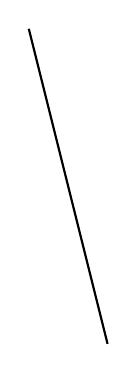
\begin{tikzpicture}
		% abscisa y ordenada
		\tkzInit[xmax=150,xstep = 50, xmin=0,ymax=250,ystep=50,ymin=0]
		\tiny\tkzLabelXY[opacity=0.6,step=1, orig=false]
		% label x, f(x)
		\tkzDrawX[opacity= .6,label=dólares,right=0.3]
		\tkzDrawY[opacity= .6,label=espacios,below = -0.6]
		%dominio y función
		\draw[domain=0:50,thick, scale=0.02] plot(\x,{200 - 4*\x}); 
	    \end{tikzpicture}
	\end{center}
	\vspace{0.5cm}

	%----------(b)
	\item ¿Qué representan la pendiente, la intersección con el eje $y$ y la intersección con el eje $x$ de la gráfica?\\\\
	    Respuesta.-\; La pendiente representa la relación de los espacios a ocuparse con respecto a los el precio en dolares del mismo, luego la intersección con el eje $x$ e $y$ representan la demanda de espacios en función al precio.\\\\ 
	    
    \end{enumerate}
	
    %--------------------15.
    \item La relación entre las escalas de temperatura Fahrenheit $(F)$ y Celsius $(C)$ está dada por la función lineal $F=\frac{9}{5}C+32$. 
    \begin{enumerate}[\bfseries (a)]
	
	%----------(a)
	\item Trace la gráfica de esta función.\\\\
	\begin{center}
	    \begin{tikzpicture}[scale=.5]
		% abscisa y ordenada
		\tkzInit[xmax=12,xstep=2,xmin=-18,ymax=33,ymin=0,ystep=2]
		\tiny\tkzLabelXY[opacity=0.6,step=1, orig=false]
		% label x, f(x)
		\tkzDrawX[opacity= .6,label=C,right=0.3]
		\tkzDrawY[opacity= .6,label=F,below = -0.6]
		%dominio y función
		\draw[domain=-17.7:5,thick, scale=.5] plot(\x,{(9/5)*\x + 32}); 
	    \end{tikzpicture}
	\end{center}
	\vspace{0.5cm}

	%----------(b)
	\item ¿Cuál es la pendiente de la gráfica y que representa? ¿Cuál es la intersección con el eje $F$ y qué representa?.\\\\
	    Respuesta.-\; La pendiente es dado por $\frac{9}{5}$ y representa la relación entre la temperatura Fahrenheit con respecto a los grados Celsius.\\
	    La intersección con el eje $F$ representa la temperatura en Fahrenheit cuando la temperatura en Celsius es $0$.\\\\ 

    \end{enumerate}

    %--------------------16.
    \item Kelly sale de Winnipeg a las $14:00$ y conduce a rapidez constante hacia el oeste a lo largo de la carretera TransCanadá. Pasa por Brandon, a $210$ km de Winnipeg, a las $16:00$.

    \begin{enumerate}[\bfseries (a)]

	%----------(a)
	\item Exprese la distancia recorrida en términos del tiempo transcurrido.\\\\
	    Respuesta.-\; Sea $t=2$ y $d=210$ entonces la función estará dada por $d(t)=105t$ ya que la relación que existe entre la distancia con respecto a tiempo  es $\dfrac{210}{2} =105$.\\\\

	%----------(b)
	\item Dibuje la gráfica de la ecuación del inciso (a).\\\\
	    Respuesta.-\; El dibujo es una función lineal.\\\\

	%----------(c) 
	\item ¿Cuál es la pendiente de esta recta? ¿Qué representa?\\\\
	    Respuesta.-\; La pendiente es $105$ y representa la relación de la distancia con respecto al tiempo.\\\\
    
    \end{enumerate}

    %--------------------17.
    \item



\end{enumerate}
